\begin{comment}
\chapter{Power Required for Vertical Climb}
\label{chap:preq}

In this chapter, the derivation for the power required in a climbing flight is explained (\autoref{eq:goodpow}). For a climbing flight, the total power required will be equal to the power required to hover plus the power required to have a certain climb speed. Since power is equal to thrust times velocity, the equation for total power required can be found in \autoref{eq:preqsum}.

\begin{equation}
\label{eq:preqsum}
    P_{req}=T\cdot V_i+T\cdot V_c
\end{equation}


In this equation, the thrust required is equal to the weight of the body plus the change in momentum of the body as can be seen in \autoref{eq:thrustreq}.

\begin{equation}
\label{eq:thrustreq}
    T=W+m\cdot a
\end{equation}

\begin{figure}[H]
    \centering
    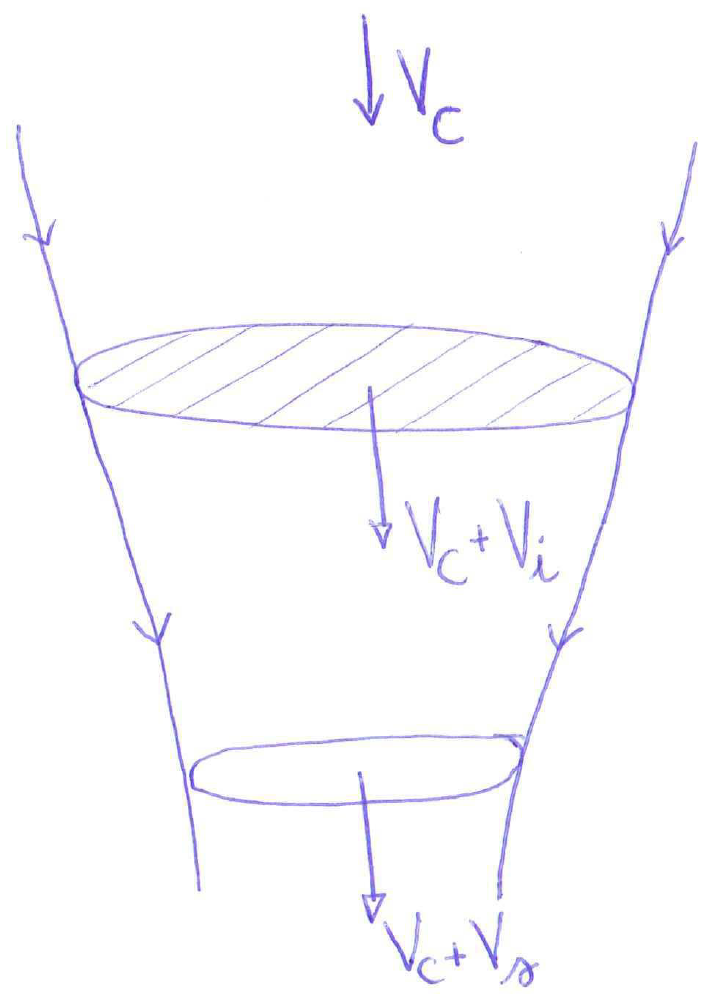
\includegraphics[width=0.3\textwidth]{Appendices/Figures/climbPreq}
    \caption{Sketch showing the flow through a propeller while climbing}
    \label{fig:engineflow}
\end{figure}

The available thrust can be calculated by multiplying the mass flow with the difference in velocity between ingoing flow and outgoing flow through the engine. As can be seen from \autoref{fig:engineflow}, the difference in velocity during a vertical climb is equal to the splitstream velocity plus the climb speed, minus the climb speed (\autoref{eq:thrustsomething}).

\begin{equation}
\label{eq:thrustsomething}
    T=\dot{m}\cdot \Delta V=\dot{m}\cdot \big((V_s+V_c)-V_c\big)
\end{equation}

The mass flow through the engine can be calculated using \autoref{eq:massflow}.

\begin{equation}
\label{eq:massflow}
    \dot{m}=\rho\cdot A\cdot \big(V_i+V_c\big)
\end{equation}

In order to find a relation between the inlet velocity and the splitstream velocity, use is made of the conservation of energy equation differentiated to time in \autoref{eq:veloc}.

\begin{equation}
\label{eq:veloc}
    \frac{\Delta W}{\Delta t} = \frac{\Delta E}{\Delta t}  \Leftrightarrow T\cdot \frac{\Delta s}{\Delta t}=T\cdot V_i=\frac{1}{2}\dot{m}{V_s}^2
\end{equation}

When  simplifying this equation and substituting \autoref{eq:thrustsomething} in this equation, the relation between $V_i$ and $V_s$ is found:

\begin{equation}
    V_s=2\cdot V_i
\end{equation}

When this is substituted in \autoref{eq:thrustsomething}, one can find an equation for $V_i$:

\begin{equation}
    V_i=-\frac{V_c}{2}\sqrt{\frac{V_c}{2}^2+\frac{T}{2\rho A}}
\end{equation}

Filling in all the relations in \autoref{eq:preqsum} yields the final total power required equation:

\begin{equation}
    P_{req} = T \cdot \bigg( \frac{V_{c}}{2} + \sqrt{ \Big( \frac{V_{c}}{2} \Big) ^2 + \frac{T}{2 \rho A}} \bigg)
\end{equation}

In order to find the power required for hovering, one can substitute $V_c = 0$ and $T = W$ into the power required equation for climbing flight:

\begin{equation}
    P_{req} = \sqrt{\frac{T^3}{2 \rho A}}
\end{equation}

\end{comment}

\chapter{References for Trendlines}

\section{References for \autoref{fig:perfthing}}
\label{sec:refvoorgev}
\begin{comment}

\begin{table}[H]
    \centering
    \caption{References used for \autoref{fig:perfthing}}
    \label{}
    \resizebox{\textwidth}{!}{\begin{tabular}{l|l}
    \multicolumn{2}{l}{http://www.iai.co.il/2013/36944-41636-en/BusinessAreas\_UnmannedAirSystems.aspx}\\
    \multicolumn{2}{l}{http://carbonix.com.au/wp-content/uploads/2017/02/17-02-22-Carbonix-VTOL-Hybrid-UAV-Information-Brochure.pdf}\\
    \multicolumn{2}{l}{http://www.textronsystems.com/what-we-do/unmanned-systems/aerosonde-commercial} \\
    https://www.quantum-systems.com/ & http://www.samcokorea.com/IMAGE/product/sub2/400.pdf \\
    http://arcturus-uav.com/product/jump-20 & 

    http://jouav.com/index.php/Jouav/index/CW20.html#parameters \\
    http://jouav.com/index.php/Jouav/index/CW10.html &

    http://www.altiuas.com/ & http://www.comquestventures.com/sr1-vtol/ \\
    http://www.dronetechuav.com/products & http://www.dronetechuav.com/products \\
    \end{tabular}}
\end{table}
\end{comment}
\section{References for \Cref{fig:costvspow,fig:costvstor}}

The references for these figures are not the full URLs, this is because multiple engines from each site has been taken. Listing all these engines would result in a very large list which does not give a better overview, nor is it more insightful.

\begin{table}[H]
    \centering
    \caption{References used for \Cref{fig:costvspow,fig:costvstor}, accessed between 15-5 and 19-5}
    \label{tab:reffig5.15.2}
    \resizebox{\textwidth}{!}{\begin{tabular}{l|l|l}
    www.evwest.com     &  www.robotshop.com & www.graupner.com\\
    www.automationtechnologiesinc.com     & www.modelmotors.cz & www.hacker-motor-shop.com \\
    www.motiondynamics.com & www.omc-stepperonline.com & www.baldor.com
    \end{tabular}}
\end{table}

\section{References for \autoref{fig:nomvalgraph}}



\begin{table}[H]
    \centering
    \caption{References used for \Cref{fig:costvspow,fig:costvstor}}
    \label{tab:reffig5.15.2}
    \resizebox{\textwidth}{!}{\begin{tabular}{l|l}
    \multicolumn{2}{l}{http://aviationweek.com/site-files/aviationweek.com/files/uploads/2015/05/Business\%20Airplane\%20Tables\_May\_2015\_revised.pdf}\\
    https://www.flyhpa.com/services/cessna/corvalis/cessna-400/ &   http://www.boeing.com/assets/pdf/commercial/airports/acaps/747\_8.pdf \\
    http://www.boeing.com/company/about-bca/index.page\%23/prices &
    http://cessna.txtav.com/en/turboprop/caravan\#\_model-specs \\
    http://www.modernairliners.com/airbus-a340-specs/ & http://www.modernairliners.com/airbus-a380/airbus-a380-specs/\\ 
    http://www.modernairliners.com/boeing-787-dreamliner/boeing-787-dreamliner-specs/
    \end{tabular}}
\end{table}

\section{References for \autoref{fig:nomcost}}


\begin{table}[H]
    \centering
    \caption{References used for \autoref{fig:nomcost}}
    \label{tab:reffigsomehting}
    \resizebox{\textwidth}{!}{\begin{tabular}{l|l}
    http://www.comquestventures.com/vertex-vtol-uas/ & https://www.birdseyeview.aero/ \\
    http://www.robotshop.com/en/xcraft-x-plusone-rtf-rc-vtol-quadcopter-hybrid.html & http://www.advancedaircraftcompany.com/hercules/ \\
    https://www.unmannedsystemssource.com/shop/vehicles/altavian-nova-f7200/ & http://www.robotshop.com/en/swift-trainer-autonomous-drone.html\#Specifications\\
    https://www.unmannedsystemssource.com/shop/vehicles/aeromapper-300/ & https://www.unmannedsystemssource.com/shop/vehicles/parrot-disco-fpv/ \\
    https://compassdrone.com/drones/swift-lynx/ & https://www.questuav.com/drones/ \\
    https://www.silvertone.com.au/sites/default/files/Silvertone\%20Flamingo\_Mk3.pdf & \\
    \end{tabular}}
\end{table}


\chapter{Task Division}
The task division will be presented in \autoref{tab:taskdivi}. The quality control was done per chapter and not per section. \\

\noindent C = Chris\\
M = Munyung\\
J = Joël \\
G = Gervase\\
O = Oscar\\
P = Piotr\\
L = Lukas\\
W = Lotte\\
K = Kelbey\\
S = Stephanie


\begin{longtable}[htb]{llp{1.5cm}p{1.5cm}p{1cm}} \label{tab:taskdivi} 
    \centering
    \caption{Task division of the mid-term report} \\
    \toprule
    \textbf{Chapter}  & \textbf{Section} & \textbf{Worked on}  & \textbf{Wrote it}  & \textbf{Checked by} \\ \midrule
    Coverpage     &        & M                   &  M                 & M                 \\ \hdashline
    Preface       &        & S                   &  S                 & L                    \\ \hdashline
    Summary       &        & S                   &  S                 & x                \\ \hdashline
    Introduction  &        & G                   &  G                 & G                    \\ \hdashline
    Project Organisation:  & Organisational Structure & W, O        & W     &  M                 \\ \hdashline
        &  Work Approach     & P, C, J, G        & P, C, J, G &               \\ \hdashline
    Revised Requirements: & Legend        & P, J     & P, J     &  M              \\ \hdashline
        &  Requirements      & P, J     & P, J     &           \\ \hdashline
    Concepts:   &  Design Option Tree & K          & K              & M \\ \hdashline
        & Feasibility Calculations & S   & S &  \\ \hdashline
        & Chosen Concepts & S & S &  \\ \hdashline
    Trade-off:  & Summary & P, K & P, K & O \\ \hdashline 
        & Trade Criteria & P, K & P, K &  \\ \hdashline
        & Criteria Weights & P, K & P, K & \\ \hdashline
        & Sensitivity Analysis &P, K & P, K & \\ \hdashline
    Performance Analysis: & Performance Trade-Off & P, G, C, J, M & P, G, C, J, M & K, O \\ \hdashline
        & Mass Estimation & P, G, C, J, M & P, G, C, J, M &  \\ \hdashline
        & Geometric Properties & P, G, C, J, M & P, G, C, J, M & \\ \hdashline
        & Performance Criteria & P, G, C, J, M & P, G, C, J, M & \\ \hdashline
    Stability \& Control: & Summary & O & O & M, K \\ \hdashline
        & Approach & L, O & L, O & \\ \hdashline
        & Concept Analysis & L, O & L, O & \\ \hdashline
        &  & & & \\ \hdashline
    Reliability Analysis: & Trade-Off & S, C  & S, C & M \\ \hdashline
        & Propulsion System & S & S & \\ \hdashline
        & Control Surfaces & S, C & S, C & \\ \hdashline
        & Wings & C & C & \\ \hdashline
    Production Cost Analysis: & Cost Trade-off & K, W & K, W & O \\ \hdashline
        & Cost Criteria & K, W & K & W \\ \hdashline
        & Nominal Values & K, W & W & K \\ \hdashline
        & Concept Analysis & K, W & K, W & \\ \hdashline
    Development Risk: & Concept Evaluation & G, J & G, J & K \\ \hdashline
        & Qualitative Concept Analysis & G, J & G, J & \\ \hdashline
    Sustainability Analysis: & Sustainability Trade-Off & M, C  & M, C & K\\ \hdashline
        & Manufacturing & M, C & M, C & \\ \hdashline
        & Noise emission & M, C & M, C & \\ \hdashline
        & Other aspects & M, C & M, C & \\ \hdashline
    Ground Handling: & Trade-Off & S & S & M \\ \hdashline
        & Criteria & S & S & \\ \hdashline
    N$^2$ Charts: & Design N2 Chart & ALL & C, W & K \\ \hdashline
        & Function N2 Chart & J, C & J & \\ \hdashline
    Sustainable Development: & Goal and Scope & M & M & x \\ \hdashline
        & Inventory Analysis & M & M & \\ \hdashline
        & Impact Analysis & M & M & \\ \hdashline
        & Interpretation & M & M & \\ \hdashline
    Technical Risk Assessment: & Risk Identification & G, S & G, S & J \\ \hdashline
        & Mapping and Mitigation of Risks & G, S & G, S & \\ \hdashline
        & Risk Mitigation & G, S & G, S &  \\ \hdashline
    Production Plan: & & P, K & P, K & K \\ \hdashline
    Operations \& Logistics: & Ground operations and logistics & O, L & L & J \\ \hdashline
        & Flight operations & O, L & L & \\ \hdashline
        & Ground station & O, L & L & \\ \hdashline
    Layout \& Configuration: & External and Internal Layout & M, P & P, J & x \\ \hdashline
        & Communication Flow & G, O & G, O & \\ \hdashline
    Verification \& Validation: & Verification & C, W & C, W & x \\ \hdashline
         & Validation & C, W & C, W & \\ \hdashline
         & Execution & C, W & C, W & \\ \hdashline
    Conclusion & & S & S & x \\ 
    \bottomrule 
\end{longtable}
